\documentclass[twoside,11pt]{article}

\usepackage[preprint]{jmlr2e}
\usepackage{amsmath}
\allowdisplaybreaks
\usepackage{enumitem}
\usepackage{pdfpages}

\makeatletter

\let\@oldsection\section
\renewcommand\section[1]{\@oldsection*{#1}}

\let\@oldsubsection\subsection
\renewcommand\subsection[1]{\@oldsubsection*{\textit{#1}}}

\let\@oldsubsubsection\subsubsection
\renewcommand\subsubsection[1]{\@oldsubsubsection*{\textit{#1}}}

\makeatother

\title{02450 Report 1}


\begin{document}

\maketitle\vspace{-3em}

\section{Table of authors and their contributions}

\begin{center}
	\begin{tabular}{| r | l | l | l |}
		\hline
				Name & Gisle Joe Garen & Ignacio Ripoll González & Sebastian Svelmøe Timm\\
		Student ID   & s242712 & s242875 & s243935\\
		\hline
		Introduction & 10\% & 80\% & 10\%\\
			  Task 1 & 10\% & 80\% & 10\%\\
			  Task 2 & 45\% & 45\% & 10\%\\
			  Task 3 & 80\% & 10\% & 10\%\\
			  Task 4 & 10\% & 10\% & 80\%\\
			Problems & 10\% & 10\% & 80\%\\
		\hline
	\end{tabular}
\end{center}


\section{Introduction}

This project focuses on the analysis of a dataset using concepts from the initial weeks of lectures on data feature extraction and visualization. In our case, the Titanic dataset is being analyzed to provide a detailed understanding and prepare it for future machine learning tasks, such as classification and regression. The report includes a description of the dataset, a summary of prior analyses, and a discussion of how various attributes might influence survival. It also addresses potential data quality issues, such as missing values and outliers, and presents visualizations, including principal component analysis (PCA), to explore patterns and relationships. This analysis serves as a foundation for evaluating the feasibility of applying machine learning techniques.


\section{Task 1: Description of the dataset}

\subsection{Explain what your data is about. I.e. what is the overall problem of interest?}

The Titanic dataset not only provides a valuable resource for statistical analysis but also offers a glimpse into one of the most infamous maritime disasters in history. The RMS Titanic set sail from Southampton, England, on April 10, 1912, bound for New York City. On board were over 2,200 passengers and crew. Tragically, on the night of April 14, 1912, the Titanic struck an iceberg and sank within a few hours. Of the more than 2,200 people on board, over 1,500 lost their lives.

The ship sank due to a combination of design flaws, including insufficient watertight compartments, and the collision with the iceberg, which breached the hull. A critical factor in the high death toll was the lack of lifeboats. The Titanic carried lifeboats for only about half of those aboard, meaning that when the ship began to sink, not everyone had a chance to escape.

The overall problem of interest in studying the Titanic dataset is to identify which demographic, socio-economic, and other relevant characteristics influenced survival rates during the disaster. The dataset includes information on passenger class, gender, age, fare, family size, and more, allowing us to analyze patterns and key factors affecting survival probabilities. It is particularly compelling because the lifeboat shortage necessitated prioritizing passengers, with those in higher social classes, such as first-class passengers, being given precedence during evacuation. By examining these factors, we can gain insights into how class, age, gender, and other variables impacted survival, revealing broader socio-economic dynamics and human behavior in life-and-death situations.

\subsection{Provide a reference to where you obtained the data.}

The Titanic dataset was obtained from Kaggle, a popular platform for data science competitions and datasets. You can access the data via the following link: \textit{Kaggle Titanic Dataset}. The data is provided in two separate datasets: one for training and one for testing. The training dataset includes the information used to build predictive models, while the testing dataset is used to evaluate the performance of these models.

\subsection{Summarize previous analysis of the data.}

In previous analyses of the Titanic dataset, several studies have explored different approaches to data preprocessing and model building. Here’s a summary of the common steps and results found in the literature:

\paragraph{Data Cleaning and Feature Engineering:} Many papers focused on addressing missing values, especially for key variables like Age, Cabin, and Embarked. Missing Age values were often imputed using the median or by predicting age based on other features like Pclass and Sex. The Cabin feature, due to its sparsity, was often dropped or transformed into a binary feature indicating whether or not the cabin number was available. Researchers frequently engineered new features, such as creating a "family size" variable by combining SibSp and Parch, or extracting titles (Mr., Mrs., Miss, etc.) from the Name attribute, which provided additional predictive power for survival models.

\paragraph{Classification Techniques:} Classification models like logistic regression, decision trees, and random forests were commonly applied to predict the survival outcome (Survived). Studies showed that factors such as Pclass, Sex, and Age were consistently among the most important predictors of survival, with women and first-class passengers having a significantly higher chance of survival.

\paragraph{Dealing with Imbalanced Data:} Given that the Titanic dataset has a higher proportion of passengers who perished (about 62\%) compared to those who survived (38\%), some studies used techniques to address this imbalance, such as oversampling the minority class (survivors) or using undersampling of the majority class (non-survivors). Advanced techniques such as SMOTE (Synthetic Minority Over-sampling Technique) were also applied to improve the performance of classification models in handling this imbalance.

\paragraph{Regression Analysis:} Some papers also performed regression analysis, focusing on predicting Fare as a continuous variable or using logistic regression to estimate the probability of survival as a function of the available features. Regression models helped identify how much socio-economic factors (e.g., Pclass, Fare, Age) contributed to survival probability.

Overall, previous studies demonstrated that proper data cleaning, feature engineering, and handling of imbalanced data significantly improved model performance. They consistently showed that social class, gender, and age were the most critical factors in determining survival, providing a clear picture of the socio-economic dynamics of the Titanic disaster.

\subsection{Explain, in the context of your problem of interest, what you hope to accomplish/learn from the data using these techniques.}
In the context of the Titanic dataset, applying classification and regression techniques will help us achieve a deeper understanding of the factors affecting survival and predict outcomes based on these factors.

\subsubsection{Classification:}

\paragraph{Objective:} The goal of classification is to predict whether a passenger survived or perished based on their characteristics.

\paragraph{Application:} We can use classification algorithms, such as logistic regression, decision trees, or support vector machines, to build a model that predicts the survival status (survived or not) of passengers in the test dataset.

\paragraph{Learning Outcome:} This will help us identify the most significant factors influencing survival, such as class, age, and gender. It will also allow us to evaluate how well these factors can predict survival and how different characteristics are weighted in the prediction process.

\subsubsection{Regression:}

\paragraph{Objective:} The goal of regression is to predict a continuous outcome based on the passenger's characteristics. In the Titanic dataset, this can be approached by predicting a variable like the fare paid by the passengers or, more creatively, estimating the probability of survival as a continuous variable.

\paragraph{Application:} We can use regression algorithms, such as linear regression, to model relationships between predictors (e.g., age, fare, family size) and the continuous outcome.

\paragraph{Learning Outcome:} This approach can reveal how numerical factors, such as the fare paid or age, correlate with survival probability or other outcomes. It can provide insights into how these continuous variables influence the likelihood of survival and offer a quantitative perspective on their impact.

\subsection{Explain which attribute you wish to predict in the regression based on which other attributes? Which class label will you predict based on which other attributes in the classification task?}

In the Titanic dataset, we can approach the classification and regression tasks as follows:

\subsubsection{Classification Task:}

\paragraph{Class Label to Predict:} Survived (a binary outcome where 0 indicates the passenger did not survive and 1 indicates survival). \\

\paragraph{Predictor Attributes:} We will predict survival based on attributes such as Pclass, Age, Sex, Fare, SibSp, Parch, and Embarked. These attributes are likely to influence whether a passenger survived the sinking of the Titanic, and analyzing their impact can provide insights into survival patterns and key factors affecting survival rates.

\subsubsection{Regression Task:}

\paragraph{Attribute to Predict:} Fare

\paragraph{Predictor Attributes:} We will predict the fare based on attributes such as Pclass (passenger class), Age, SibSp (number of siblings/spouses aboard), Parch (number of parents/children aboard), Sex, and Embarked (port of embarkation). These predictors can help us understand how different factors influence the fare a passenger paid.

By using these attributes in classification and regression, we aim to build models that can predict the survival status and fare of passengers, respectively, based on their characteristics and other relevant information.

\subsection{If you need to transform the data in order to carry out these tasks, explain roughly how you plan to do this.}
To effectively carry out the classification and regression tasks, we will need to transform the Titanic dataset to address various quality issues and prepare it for analysis. Here’s a rough plan for transforming the data:

\begin{itemize}
    \item \textbf{Handling Missing Values:}
    \begin{itemize}
        \item \textit{Age:} Fill missing values using imputation techniques such as the mean or median age, or use more sophisticated methods like predicting age based on other attributes (e.g., passenger class and title).
        \item \textit{Embarked:} Fill missing values with the most common port of embarkation or use imputation based on other features.
        \item \textit{Cabin:} Since the cabin feature is sparse, we might consider dropping it or extracting and using only the information about whether a cabin was known or not.
    \end{itemize}
    \item \textbf{Standardizing and Encoding:}
    \begin{itemize}
        \item \textit{Categorical Variables:} Convert categorical variables like Sex, Embarked, and Pclass into numerical format using techniques such as one-out-of-K encoding or label encoding. For example, Sex can be converted into binary (0 for male, 1 for female), and Embarked can be one-out-of-K encoded into separate columns for each port of embarkation.
        \item \textit{Passenger Name:} This feature can be dropped or used to extract titles (e.g., Mr., Mrs., Miss) that might provide additional insights.
    \end{itemize}
    \item \textbf{Handling Outliers:}
    \begin{itemize}
        \item \textit{Fare:} Check for outliers in the Fare attribute and decide whether to remove or transform them. For instance, applying a log transformation might help normalize the distribution.
    \end{itemize}
    \item \textbf{Feature Engineering:}
    \begin{itemize}
        \item \textit{Family Size:} Combine SibSp and Parch to create a new feature representing the total family size aboard.
        \item \textit{Title Extraction:} Extract titles from the Name attribute to create a feature that might be useful for predicting survival.
    \end{itemize}
    \item \textbf{Normalization and Scaling:}
    \begin{itemize}
        \item \textit{Numerical Features:} Scale numerical features like Age and Fare to ensure they are on a comparable scale, which can improve the performance of many machine learning algorithms.
    \end{itemize}
    \item \textbf{Data Splitting:}
    \begin{itemize}
        \item \textit{Train-Test Split:} Ensure proper splitting of the dataset into training and testing sets for validation of the models.
    \end{itemize}
\end{itemize}

By addressing these data quality issues and performing these transformations, we will prepare the dataset for accurate and meaningful analysis, enabling us to build effective regression and classification models.


\section{Task 2: Data Attribute Description and Issues}

\subsection{Attribute Types and Measurement Scales}
This section provides a detailed explanation of the attributes in the Titanic dataset, categorizing each as discrete or continuous and identifying their corresponding measurement scales: Nominal, Ordinal, Interval, or Ratio. Understanding the nature of these variables is essential for selecting the appropriate analysis techniques in subsequent stages.

THIS IS A REFERENCE \ref{table:description}.

Each of these attributes serves a distinct role in analysis, with discrete variables often used for classification and categorical comparisons, and continuous variables applied in regression or to explore relationships like fares and age.

\subsection{Data Quality Issues}
The Titanic dataset contains several data quality issues that must be addressed before analysis. The primary problems identified are as follows:

\subsubsection{Missing Values}
\begin{itemize}
    \item \textbf{Age:} A significant number of passengers have missing values for the Age attribute, which could impact the analysis of age as a factor in survival.
    \item \textbf{Cabin:} The Cabin attribute has a large proportion of missing values, making it difficult to use for meaningful analysis. In many cases, this variable is either dropped or transformed into a binary feature (whether a cabin number was recorded or not).
    \item \textbf{Embarked:} A few missing values are present in the Embarked attribute, which indicates the port of boarding.
\end{itemize}

\subsubsection{Corrupted or Inconsistent Data}
\begin{itemize}
    \item \textbf{Ticket:} The Ticket attribute consists of alphanumeric codes with no consistent format, leading to difficulty in interpreting this feature. It may need to be treated as a nominal attribute or disregarded altogether.
    \item \textbf{Fare:} There are potential outliers in the Fare attribute, as some values seem unusually high or low, which could skew the analysis if not handled properly.
\end{itemize}

\subsubsection{Data Standardization}
\begin{itemize}
    \item \textbf{Name:} The Name attribute contains titles (e.g., Mr., Mrs., Miss) embedded within full names. Extracting the title could be useful for analysis, but without standardization, this information is not immediately usable.
\end{itemize}

These data issues highlight the need for preprocessing steps, such as handling missing values, addressing outliers, and standardizing certain attributes, to ensure the dataset is ready for analysis.


\section{Task 3}


TBD


\section{Task 4}

TBD

\section{Exam Problems}

\subsection{Question 1}

The only correct statement is C. The justification is:

\begin{itemize}
\item
  The variable \(x_1\) represents the time of day in blocks of 30
  minutes that partition a day into a finite number of intervals. The
  variable is therefore discrete. Since the intervals can be ordered,
  the variable is ordinal.
\item
  The attribute \(x_6\) is a ratio variable. The number of broken
  traffic lights is clearly a numeric variable. The cannonical zero of
  the variable is zero broken traffic lights.
\item
  The attribute \(x_7\) is a ratio variable for much the same reasons as
  for \(x_6\).
\item
  The congestion level is ordinal as it is a discrete variable that can
  be ordered.
\end{itemize}

The statements A, B, and D are all incorrect as they mistake \(x_1\) for something other than an ordinal variable.

\subsection{Question 2}

\begin{enumerate}[label=\Alph*.]
	\item This statement is correct since \(|26 - 19| = 7\) and that is the maximal difference among the respective coordinates of the two vectors.

	\item The metric is
	\[
		d_3(x_{14}, x_{18}) = \sqrt[3]{|26 - 19|^3 + |2 - 0|^3} \approx 7.05.
	\]
	Thus, the statement is incorrect.

	\item The metric is
	\[
		d_1(x_{14}, x_{18}) = |26 - 19| + |2 - 0| = 9.
	\]
	Thus, the statement is incorrect.

	\item The metric is
	\[
		d_4(x_{14}, x_{18}) = \sqrt[4]{|26 - 19|^4 + |2 - 0|^4} \approx 7.01.
	\]
	Thus, the statement is incorrect.

\end{enumerate}

\subsection{Question 3}

\begin{enumerate}[label=\Alph*.]
	\item The explained variance is
	\[
		\frac{13.9^2 + 12.47^2 + 11.48^2 + 10.03^2}{13.9^2 + 12.47^2 + 11.48^2 + 10.03^2 + 9.45^2} \approx 0.87.
	\]
	The statement is therefore correct.

	\item The explained variance is
	\[
		\frac{11.48^2 + 10.03^2 + 9.45^2}{13.9^2 + 12.47^2 + 11.48^2 + 10.03^2 + 9.45^2} \approx 0.48.
	\]
	Thus, the statement is incorrect.

	\item The explained variance is
	\[
		\frac{13.9^2 + 12.47^2}{13.9^2 + 12.47^2 + 11.48^2 + 10.03^2 + 9.45^2} \approx 0.52.
	\]
	Thus, the statement is incorrect.

	\item The explained variance is
	\[
		\frac{13.9^2 + 12.47^2 + 11.48^2 + 10.03^2 + 9.45^2}{13.9^2 + 12.47^2 + 11.48^2 + 10.03^2 + 9.45^2} \approx 0.72.
	\]
	Thus, the statement is incorrect.

\end{enumerate}

\subsection{Question 4}

\begin{enumerate}[label=\Alph*.]
	\item Such an observation will typically have a negative value as the high values of the third and fourth coordinates will make the negative coordinates of the principal component dominate. The statement is false.

	\item For much the same reasons as in A, such an observation will typically have a negative value. This statement is false.

	\item For such an observation, the positive value of the second coordinate of the principal component will dominate the sum in the dot product. The value will therefore typically be positive. The statement is false.

	\item The only negative coordinate of the principal component is the first one. As the observation has a low value in this position, and high values everywhere else, the dot product will typically be positive. The statement is correct.
	\end{enumerate}

\subsection{Question 5}

We are given the following data:
\[
	n = 20000, M_{11} = 2, M_{01} = 5, M_{10} = 6.
\]
The Jaccard similarity of the documents is
\[
	\frac{M_{11}}{M_{11} + M_{01} + M_{10}} \approx 0.1538.
\]
The correct answer is A.

\subsection{Question 6}

The probability \(p(\hat{x}_2 = 0 \, | \, y = 2)\) can be found by marginalizing on \(\hat{x}_7\). This results in the probability
\[
	p(\hat{x}_2 = 0 \, | \, y = 2) = p(\hat{x}_2 = 0, \hat{x}_7 = 0 \, | \, y = 2)
	+ p(\hat{x}_2 = 0, \hat{x}_7 = 1 \, | \, y = 2) = 0.81 + 0.03 = 0.84.
\]
The correct answer is B.

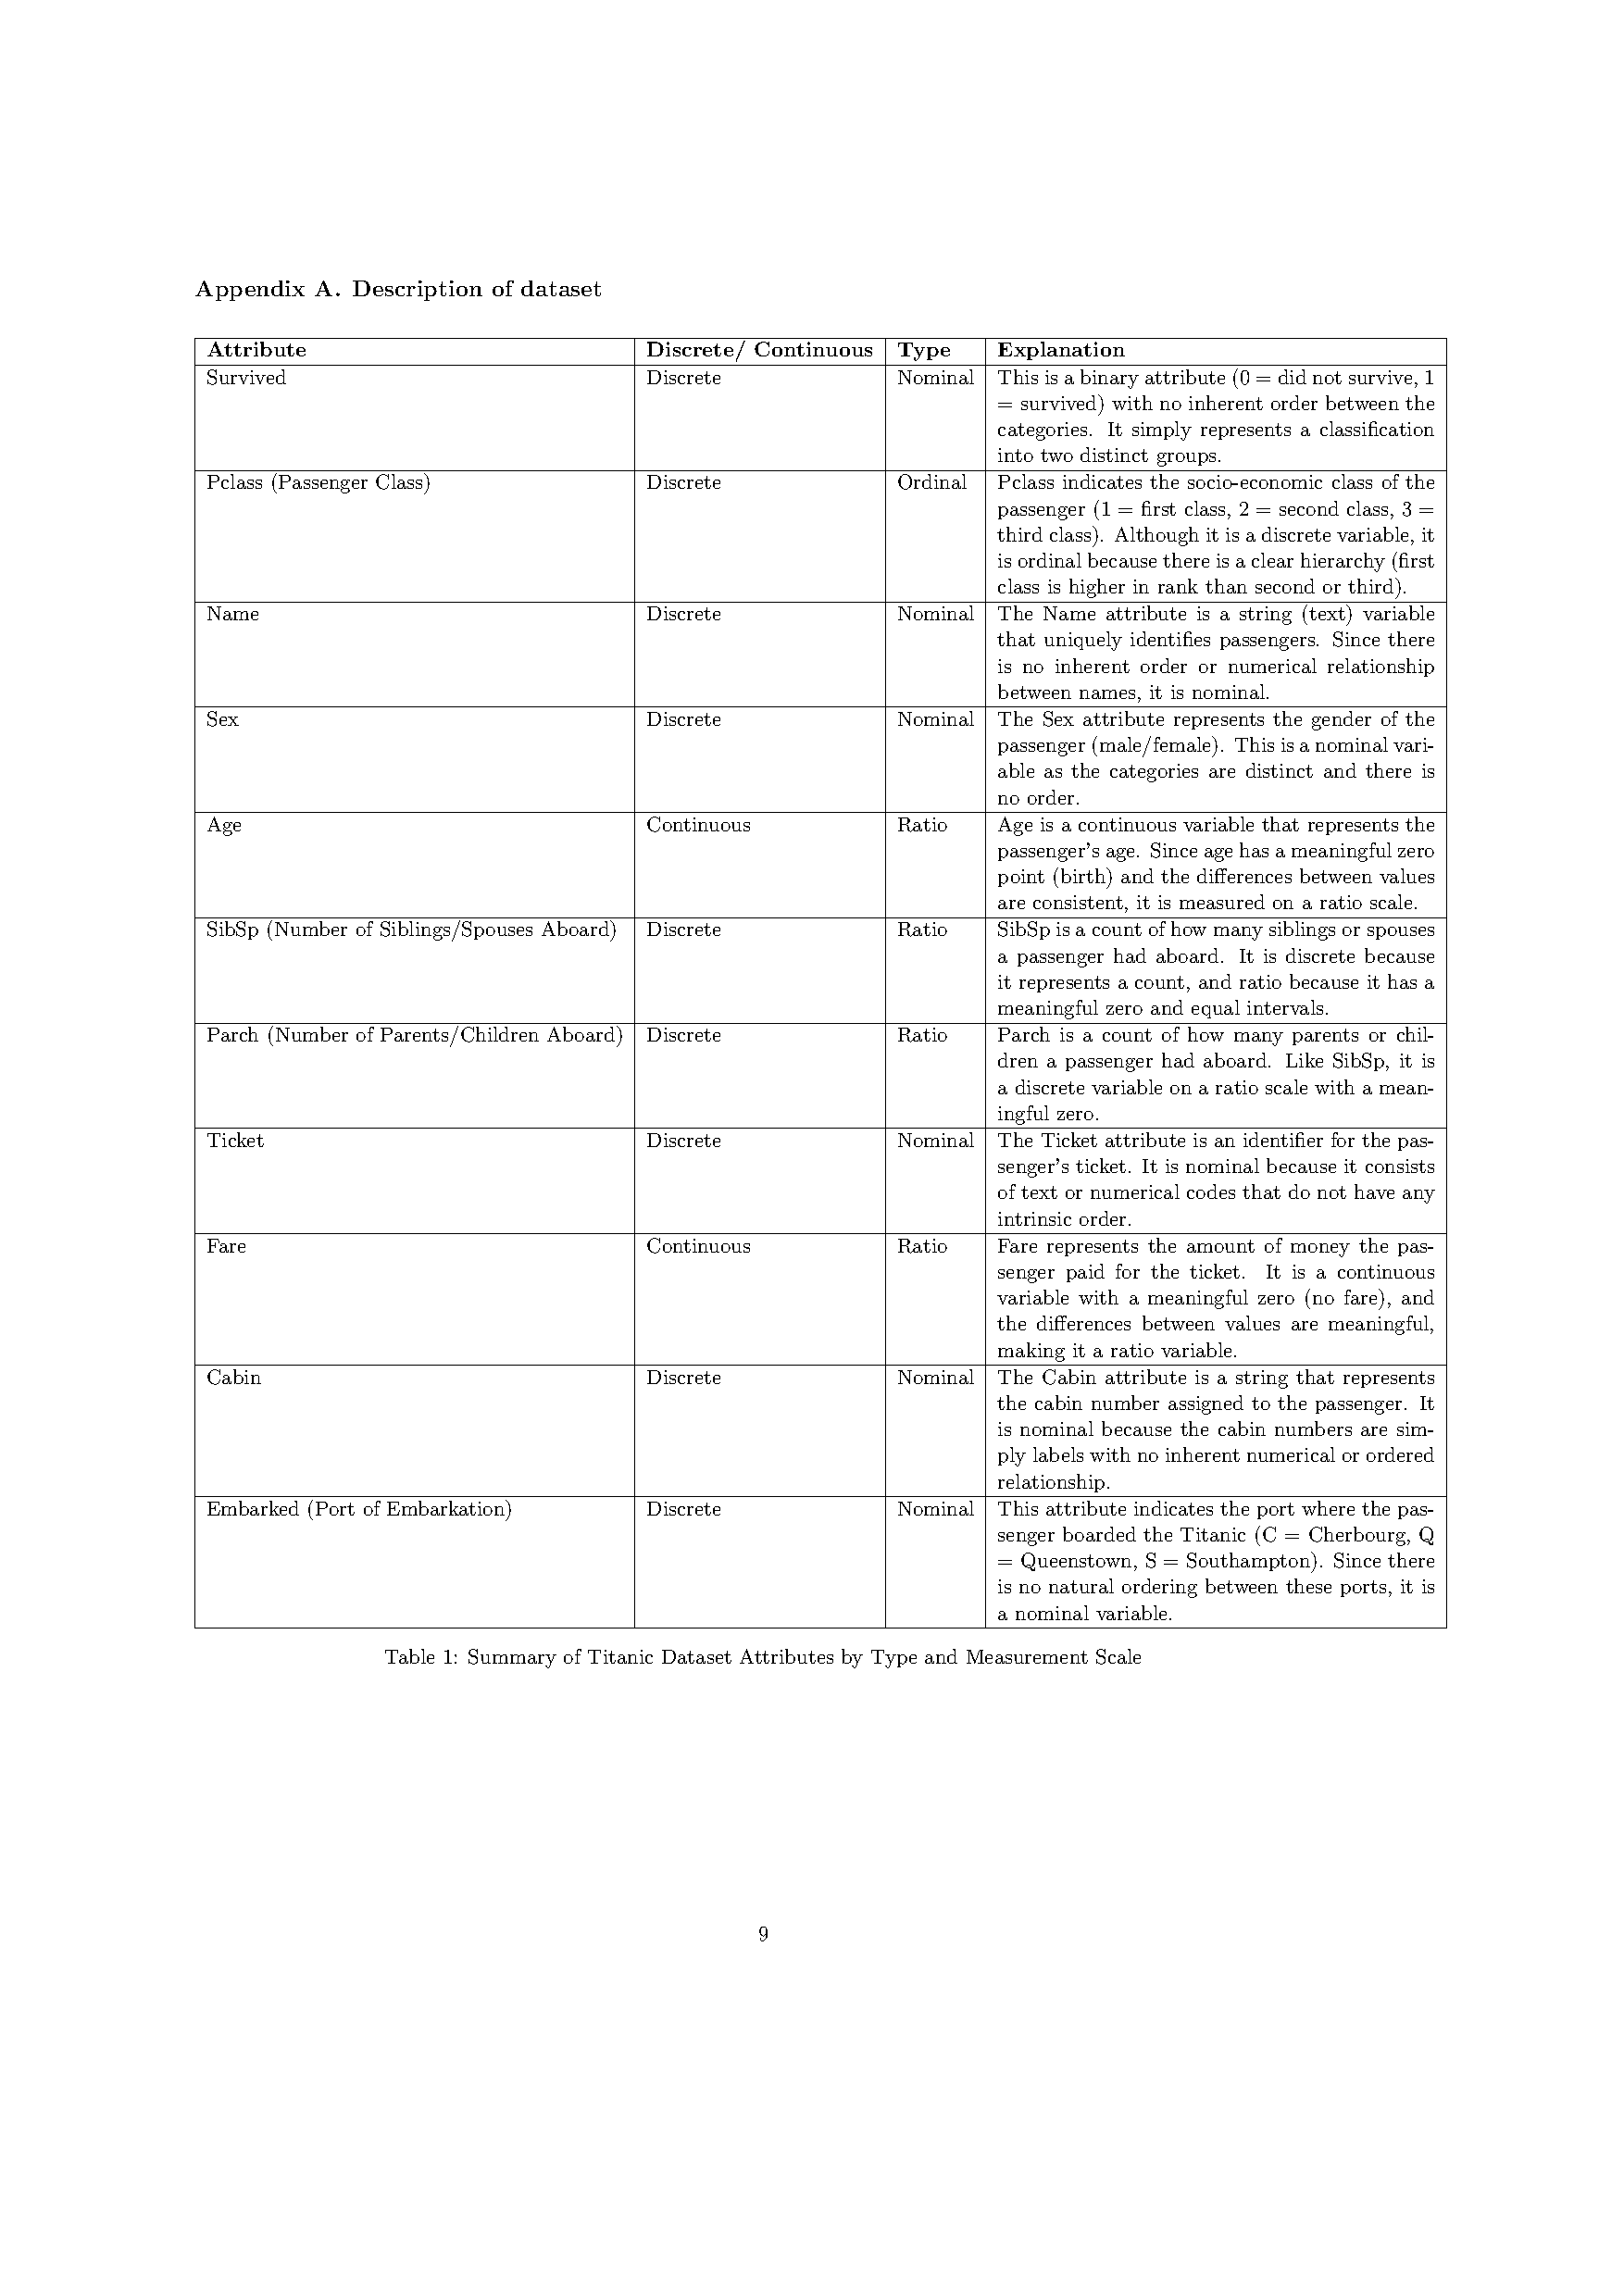
\includepdf[pages=1,fitpaper=true,addtolist={%
	1,%
	table,%
	A test figure included with the help of the \texttt{pdfpages} package,%
	table:description%
}]{table}

\end{document}
